\documentclass{article}
\usepackage{url}
\usepackage{amsmath,bm}
\usepackage{amsfonts}
\pagestyle{empty}
\setlength{\textwidth}{7in}
\setlength{\oddsidemargin}{-.5in}
\setlength{\evensidemargin}{-.5in}
\setlength{\topmargin}{-.75in}
\setlength{\textheight}{9.25in}

\usepackage{Sweave}
\begin{document}

\begin{center}
{\bf STAT 515}

{\bf Homework \#4 WITH SOLUTIONS}
\end{center}

\begin{enumerate}

\item Suppose that in a branching process with $X_0=1$, each individual produces
some number of offspring that is Poisson with mean 1, independently of all other
individuals.

  \begin{enumerate}

  \item What is the expected number of generations until the process either dies
  out or attains size $X_n\ge 5$?
  \begin{quotation}{\bf Solution:}
  This is a question we'll use R to solve.  Let us first define a Markov chain on the states
  $\{0, 1, \ldots, 5\}$, where 0 and 5 are absorbing states.  If $X_n=i$, where $1\le i\le 4$,
  then we know that $X_{n+1}$ will be the sum of $i$ independent Poission$(1)$ variables,
  which is Poisson$(i)$.  To construct the transition matrix, therefore, we must simply be careful
  to make the last column equal to $P(X_{n+1} \ge 5 \mid X_n=i)$:
\begin{Schunk}
\begin{Sinput}
> P <- diag(rep(1, 6))
> for(i in 1:4) 
+   P[i+1, ] <- c(dpois(0:4, i), 1-ppois(4, i))
> print(P)
\end{Sinput}
\begin{Soutput}
           [,1]       [,2]      [,3]       [,4]       [,5]        [,6]
[1,] 1.00000000 0.00000000 0.0000000 0.00000000 0.00000000 0.000000000
[2,] 0.36787944 0.36787944 0.1839397 0.06131324 0.01532831 0.003659847
[3,] 0.13533528 0.27067057 0.2706706 0.18044704 0.09022352 0.052653017
[4,] 0.04978707 0.14936121 0.2240418 0.22404181 0.16803136 0.184736755
[5,] 0.01831564 0.07326256 0.1465251 0.19536681 0.19536681 0.371163065
[6,] 0.00000000 0.00000000 0.0000000 0.00000000 0.00000000 1.000000000
\end{Soutput}
\end{Schunk}
  Now that we have found $P$, let us calculate $S=(I-P_T)^{-1}$, where $P_T$ is the
  sub matrix corresponding only to the transient states:
\begin{Schunk}
\begin{Sinput}
> S <- solve(diag(rep(1, 4)) - P[2:5, 2:5])
> print(S)
\end{Sinput}
\begin{Soutput}
          [,1]      [,2]      [,3]      [,4]
[1,] 1.9584153 0.6375343 0.3487308 0.1816200
[2,] 0.9877498 1.8772188 0.6040866 0.3554605
[3,] 0.7807759 0.7930153 1.6475972 0.4478620
[4,] 0.5477606 0.5924388 0.5417979 1.4328109
\end{Soutput}
\end{Schunk}
  Since $X_0=1$, the relevant row of $S$ is the first row, which gives the expected number of time
  steps spent in each of the four transient states of the chain.  Since we want to know the expected
  number of generations spent in all transient states combined (since it must either die out or
  attain $X_n\ge 5$ after it leaves the class of transient states), our solution equals
\begin{Schunk}
\begin{Sinput}
> sum(S[1,])
\end{Sinput}
\begin{Soutput}
[1] 3.1263
\end{Soutput}
\end{Schunk}
  \end{quotation}

  \item What is the probability that the process will ever attain size $X_n\ge 5$?  
  \begin{quotation}{\bf Solution:}
  One way to approach this question is numerically.
  Consider the effect of running this Markov chain for $2^{15}=32,768$ steps:
\begin{Schunk}
\begin{Sinput}
> PP <- P
> for (i in 1:15) PP <- PP %*% PP # square the matrix 15 times
> print(PP)
\end{Sinput}
\begin{Soutput}
          [,1] [,2] [,3] [,4] [,5]      [,6]
[1,] 1.0000000    0    0    0    0 0.0000000
[2,] 0.8274304    0    0    0    0 0.1725696
[3,] 0.6540130    0    0    0    0 0.3459870
[4,] 0.4847863    0    0    0    0 0.5152137
[5,] 0.3349051    0    0    0    0 0.6650949
[6,] 0.0000000    0    0    0    0 1.0000000
\end{Soutput}
\end{Schunk}
  Of course, the zeros in the above matrix are not exactly zero, but they are so small 
  (on my machine, smaller than about $10^{-324}$) that R simply rounds
  them to zero.
  Clearly multiplying the above matrix by $P$ gives the above matrix,
  so we can see that each additional step won't change the probabilities of attaining the various
  states in the long run.
  Since $X_0=1$, we should consider the second row of the above matrix to find the 
  resulting distribution over the six states after running the chain for a long time.  
  We conclude that the answer is given by:
\begin{Schunk}
\begin{Sinput}
> PP[2,6]
\end{Sinput}
\begin{Soutput}
[1] 0.1725696
\end{Soutput}
\end{Schunk}
  \end{quotation}

  \end{enumerate}

\item Define a Markov chain on the nonnegative integers as follows:
$P_{0j}=I\{j=1\}$, and for $i>0$,
\begin{eqnarray*} 
P_{ij}&=& 
  \begin{cases} 
  i/(i+1) & \mbox{if $j=i+1$} \\ 
  1/(i+1) & \mbox{if $j=0$}\\ 0 & \mbox{otherwise.} 
  \end{cases} 
\end{eqnarray*}

  \begin{enumerate}
  
  \item Argue that this chain is irreducible and aperiodic.
  \begin{quotation}{\bf Solution:}
  For $i<j$, it is always possible to move $i\to i+1 \to \cdots \to j-1 \to j$ 
  with positive probability.  Furthermore, it is possible to move $j\to 0 \to 1 \to \cdots \to i-1 \to i$.
  This proves irreducibility.  Since period is a class characteristic, proving that the whole chain
  is aperiodic is equivalent to proving that any specific state is aperiodic.  Since it is possible 
  to move from $1\to 2 \to 0 \to 1$ and also from $1\to 0 \to 1$, we know that the period of 
  state 1 must be a divisor of both 3 and 2.  The only such integer is 1, so state 1 must have
  period 1, which makes the whole chain aperiodic.
  \end{quotation}

  \item Prove that all states are recurrent.
  \begin{quotation}{\bf Solution:}
  Since recurrence is a class characteristic,
  it suffices to check that state zero is recurrent.  We could try to check
  $\sum_{n=1}^\infty P_{00}^n=\infty$, but it may be easier to verify directly that 
  \[
  P(\mbox{$X_n=0$ for some $n>0$} \mid X_0=0) = 1,
  \]
  as required by the definition.  To do this, let us calculate directly
  \begin{eqnarray*}
  f_n &=&  P(\mbox{$n>0$ is the smallest time when $X_n=0$}  \mid X_0=0) \\
  &=& \frac{1}{n(n-1)} \mbox{for $n\ge2$}.
  \end{eqnarray*}
  (To see this, just notice the pattern:  $f_1=0$, $f_1=\frac12$,
  $f_2=\frac12 \frac13$, $f_3=\frac12\frac23 \frac14$, $f_4=\frac12 \frac23 \frac34 \frac15$, etc.)
  It is easy to prove, e.g. by induction, that
  \[
  \frac{1}{2\times 1} +   \frac{1}{3\times 2} +   \cdots +   \frac{1}{n\times (n-1)} = \frac{n-1}{n}.
  \]
  Therefore, the limit of this sum as $n\to\infty$ equals one, which means that $X_n$ will be
  back in state zero for some $n>0$ with probability one.
  \end{quotation}

  \item Prove that all states are null recurrent. (You may assume without proof
  that null recurrence is a class property.)
  \begin{quotation}{\bf Solution:}
  Using the $f_n$ quantities from part (b), we may easily verify that the expected time to return to state 0, starting
  in state zero, is not finite:
  \[
  E(\mbox{time until return}) = \sum_{n=1}^\infty nf_n = \sum_{n=2}^\infty \frac{1}{n-1} = \infty.
  \]
  Since state 0 is therefore null recurrent, all states are null recurrent.
  \end{quotation}

  \end{enumerate}
  
\item Consider the symmetric one-dimensional random walk of Example 4.15 with
$p=1/2$.

  \begin{enumerate}
  
  \item Let $T_{i}$ be the time at which the random walk first revisits state
  $i$ given that it begins in state $i$. That is, $T_{i} = \inf \{n>0: X_n=i
  \mid X_0=i\}$. For any $n>0$, find $P(T_i=2n)$.
   
  {\bf Hint:\ } Read the ballot problem example of Section~3.5 and the
  discussion following it.
   
  \begin{quotation}{\bf Solution:}
  Since $P(T_i=2n)$ is the same as the probability that the $(2n)$th flip is the first time we have the same number of
  heads and tails if we flip a fair coin repeatedly, the argument following the ballot problem example shows that
  \[
  P(T_i=2n) = \frac{ {{2n}\choose n} \left(\frac12\right)^{2n} }{2n-1}.
  \]
  \end{quotation}

  \item Prove that all states are null recurrent by showing that
  $E(T_i)=\infty$.
   
  {\bf Hint:\ } Read the random walk example of Section~4.3 for an idea about
  how to show this.

  \begin{quotation}{\bf Solution:}
  Since $T_i$ cannot be odd, the result of part (a) gives
  \[
  E(T_i) = \sum_{n=1}^\infty 2n P(T_i=2n) = \sum_{n=1}^\infty \frac{ n {{2n}\choose n}}{2^{2n}(2n-1)}.
  \]
  As the book states, when $a_n\sim b_n$ as $n\to\infty$, we can claim $\sum_na_n=\infty$ whenever $\sum_nb_n=\infty$.
  Using Stirling's approximation, we find that
  \[
  \frac{ n {{2n}\choose n}}{2^{2n}(2n-1)} \sim
  \frac{n4^n}{\sqrt{\pi n} 4^n(2n-1)} = \frac{\sqrt{n} }{\sqrt{\pi} (2n-1)} \sim \frac{ 1}{2\sqrt{\pi n}}.
  \]
  Since $\sum_{n=1}^\infty 1/\sqrt{n}=\infty$, we conclude that $E(T_i)=\infty$.
  \end{quotation}

  \end{enumerate}

\item Read the random walk example of Section~4.8 and the discussion of the
Ehrenfest model following it.

  \begin{enumerate}

  \item Simulate the simple Ehrenfest diffusion process with total number of
  particles $M=30$. Start the process at $X_0=10$. Run the process for 100,000
  steps and draw a histogram of the resulting values of $X_t$.
  \begin{quotation}{\bf Solution:}
  As explained in the textbook, the Ehrenfest process may be envisioned as two 
  containers, with $X_n$ giving the total number of particles in the first container
  at time $n$.  At each step, we select one particle at random and switch it to the
  other container.  Alternatively, we let $X_{n+1}=X_n + (1- 2Y_n)$, where 
  $Y_n$ is Bernoulli with parameter $X_n/30$.
\begin{Schunk}
\begin{Sinput}
> X <- rep(0, 100001) # This is where we will store all the states in the chain
> X[1] <- 10 # Initialize first state to 10
> for (i in 1:100000) {
+   X[i+1] <- X[i] + 1 - 2 * rbinom(1, 1, X[i]/30)
+ }
> # Now produce the histogram.  
> # Sweave will automatically put the figure into the LaTeX document!
> breaks <- ((min(X)-1):max(X)) + 0.5
> hist(X[-1], breaks=breaks, main="Problem 4(a) and (b)") 
> # Here is part (b):
> vals <- min(X):min(30, max(X)) # technically, the binomial can't go higher than n
> lines (vals, 100000*dbinom(vals, 30, 1/2), # dbinom is the binomial mass function
+        col = 2, # make the lines red
+        lwd = 2, # change line width to make the lines more visible
+        lty = 2, # change line type to dotted
+        type= "b") # type "b" means o--o--o--o style
\end{Sinput}
\end{Schunk}
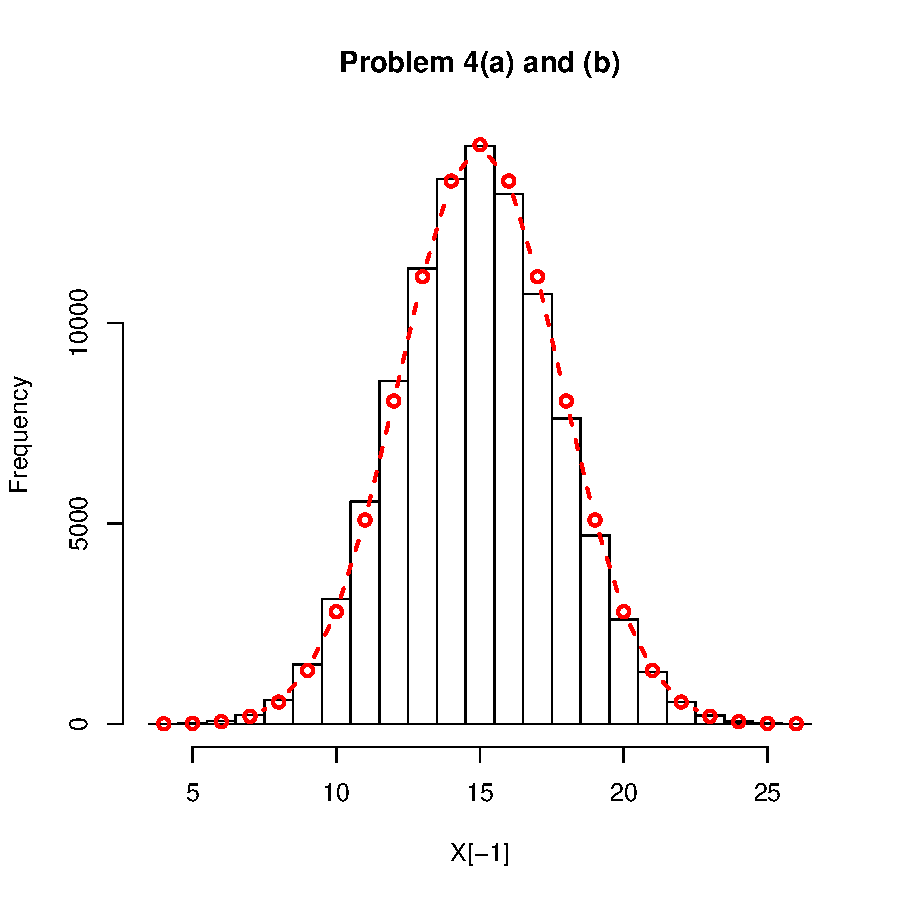
\includegraphics{sol04-006}
  \end{quotation}

  \item On the same histogram, indicate the true values that would be expected
  from a sample of size 100,000 from a binomial$(n=30, p=1/2)$ distribution.  See
  the example R code for ideas on how to do this.
  \begin{quotation}{\bf Solution:}
  This is done in the code for part (a).
  \end{quotation}

  \item Explain what you observe from the comparison in part (b). Is the Markov
  chain you are simulating ergodic?
  \begin{quotation}{\bf Solution:}
  Clearly, the observed frequencies are very close to the theoretical stationary probabilities.
  This chain has period 2, so it is not ergodic.
  \end{quotation}

  \end{enumerate}

\item Let $Q$ be a transition ``matrix'' for an irreducible Markov chain on the
set $\mathbb{Z}$ of all integers; i.e., $Q_{ij}=P(X_n=j \mid X_{n-1}=i)$ for all
$i,j\in\mathbb{Z}$. Assume that $Q_{ij}>0$ if and only if $Q_{ji}>0$ and that
$Q_{ii}>0$ for all $i$. Also suppose that
\[
\sum_{i \in \mathbb{Z}} \pi_i = 1 \quad \mbox{and $\pi_i>0$ for all
$i\in\mathbb{Z}$}
\]
and define
\[
\alpha(i,j) = \min\left(\frac{\pi_jQ_{ji}}{\pi_iQ_{ij}}, 1\right) \quad\mbox{for
all $i,j\in\mathbb{Z}$.}
\]
Consider a second Markov chain with transition probabilities given by
\[
P_{ij} =  
  \begin{cases}
  \alpha(i,j) Q_{ij} &  \mbox{ if  $ j \neq i$}  \\
  Q_{ii} + \sum_{k\neq i} Q_{ik}(1-\alpha(i,k)) & \mbox{if $i=j$,}
  \end{cases}
\]
Using time reversibility arguments, show that the second Markov chain has
stationary probabilities $\{\pi_i\}$ and that these stationary probabilities are
also the limiting probabilities of the Markov chain.
  \begin{quotation}{\bf Solution:}
  Since $Q$ is irreducible, then $P$ must
  also be irreducible:  Given any $i$ and $j$, there is a path with positive probability
  from $i$ to $j$ and another
  from $j$ to $i$ under $Q$, and since $\alpha(i,j)$ must be nonzero whenever 
  $Q_{ij}$ is, we conclude that the same paths have positive probability under $P$.
  Also, since $P_{ii}\ge Q_{ii}>0$ for all $i$, the $P$ chain is aperiodic.  
  
  Let us now demonstrate that the $P$ chain satisfies detailed balance with the $\pi$ vector.  
  This will imply in turn that the $\pi$ matrix is a stationary probability, which means that the chain
  is positive recurrent, so that the chain is ergodic and we are done.  For any $i\ne j$, 
  we prove detailed balance by considering three cases:
  \begin{itemize}
  \item If $Q_{ij}=Q_{ji}=0$, then $P_{ij}=P_{ji}=0$ and $\pi_iP_{ij}=\pi_jP_{ji}$ is trivial.
  \item If $\pi_jQ_{ji}\ge \pi_iQ_{ij}$, then $\alpha(i,j)=1$ and $\alpha(j,i)=\pi_iQ_{ij}/(\pi_jQ_{ji})$. Therefore,
  \[
  \pi_jP_{ji} = \pi_j \frac{\pi_i Q_{ij} }{\pi_j Q_{ji}} Q_{ji} = \pi_i Q_{ij} = \pi_iP_{ij}.
  \]
  \item If $\pi_jQ_{ji}\le \pi_iQ_{ij}$, then $\alpha(j,i)=1$ and $\alpha(i,j)=\pi_jQ_{ji}/(\pi_iQ_{ij})$. Therefore,
  \[
  \pi_iP_{ij} = \pi_i \frac{\pi_j Q_{ji} }{\pi_i Q_{ij}} Q_{ij} = \pi_j Q_{ji} = \pi_jP_{ji}.
  \]
  \end{itemize}  
  \end{quotation}

\item The lifetimes of two machines are independent with exponential
distributions with rates $\lambda_1$ and $\lambda_2$, respectively. Suppose
machine 1 starts working now and machine 2 starts working $t$ units of time
later. What is the probability that machine 1 will fail before machine 2?
  \begin{quotation}{\bf Solution:}
  With probability $1-e^{-\lambda_1 t}$, machine 1 will fail before $t$ and therefore certainly
  before machine 2.  
  On the other hand, if machine 1 lasts until at least $t$, then the memoryless property means that
  it's just as if both machines started at the same time, in which case machine 1 fails first
  with probability $\lambda_1/(\lambda_1+\lambda_2)$ (as we've shown in class). 
  Therefore, the answer follows by conditioning on whether machine 1 fails before time $t$:
  \[
  1-e^{-\lambda t} + e^{-\lambda t} \left( \frac{\lambda_1}{\lambda_1 + \lambda_2} \right) =
  1 - e^{-\lambda t} \left( \frac{\lambda_2}{\lambda_1 + \lambda_2} \right).
  \]
  \end{quotation}

\end{enumerate}

\end{document}

